\section{Empirical Results}
In this section, we will show our empirical results about the relation between each of the 4 metrics BLEU, SED, TREED, GVED with Semantic Score. We use Pearson\rq s correlation coefficient to gauge their relations. 
\subsection{RQ1: BLEU vs Semantic}
Figures \ref{fig:BleuSemlpSMT}, \ref{fig:BleuSemMppSMT}  show the scatter plots between 2 metrics: BLEU and Semantic. Each point represents scores of a pair of methods where its x-axis value is BLEU score and y-axis value is Semantic score.
The correlation coefficient between BLEU and Semantic score for the model mppSMT is 0.524 and for the model lpSMT is 0.67. That meant there is a positive relationship between the 2 metrics, but it is not strong since the correlation is closer to 0.5 than to 1.0. The graphs in the figures \ref{fig:BleuSemlpSMT} and \ref{fig:BleuSemMppSMT}  also demonstrate the weak correlation.

\emph{Observation 1:} For a fixed value of Semantic score, there can be many associated BLEU values. Specifically, in the model lpSMT, with a Semantic Score of 1, the BLEU scores can be varied greatly between 0-1, which was reflected on the top horizontal line of dots in figure \ref{fig:BleuSemlpSMT}. Similarly, in the figure \ref{fig:BleuSemMppSMT}, with a Semantic Score of 1, the BLEU scores are in the range of 0.5 to 1. 

\emph{Observation 2:} For a fixed value of BLEU, there can be many associated Semantic scores. For an instance, the figure \ref{fig:BleuSemMppSMT} shows that for a high BLEU score, for example 0.8, can have Semantic Score from 0.25 to 1. This can be observed by the vertical line of dots in the figure. 

\emph{Implication 1: }From observation 1, it can be implied that a translated method can have low BLEU score, but high Semantic score. This can be explained by the situations in which translated method uses different code structure to perform the same functionality. For example, the translated method that got maximum Semantic score (raw score is 4, normalized score is 1) on figure \ref{fig:scoreEG} has low BLEU score (0.4) because it uses a normal \lq for\rq  loop instead of a \lq for each\rq  loop as the reference code does. Moreover, there is also the white space problem. For example, the translated method has tokens: \lq m()\rq, but the reference method has: \lq m ()\rq. This situation reduces n-grams precision, but the human subject will still evaluate the result with high Semantic score.     

\emph{Implication 2: }From observation 2, a translated method can have high BLEU score, but low Semantic score. The reason of this implication is that BLEU does not take into consideration order of n-grams tokens. So if a translated method has multiple correct n-grams tokens, but in the wrong order, the method can still be justified as not useful by human judgment. For example, in figure \ref{fig:issueexample2} the translated method misplaces the position of the bracelet which makes the method has low Semantic score, but high BLEU score. Another reason for this implication is that resulting method does not capture the important program elements. For example, the result contains mostly key words and punctuation like \lq if\rq, \lq public\rq, \lq()\rq, but miss out important program elements like function calls or variable names. In this case, it will have low Semantic score while moderate to high BLEU score. 

The two implications above shows that an improvement in BLEU is not sufficient nor necessary to improve translation migration quality. In conclusion, BLEU does not reflect well the semantics of source code, as well as is not suitable to use to evaluate semantic accuracy for SMT-based Code Migration system.

 
\begin{figure}
\caption{BLEU vs Semantic (lpSMT)}
\centering
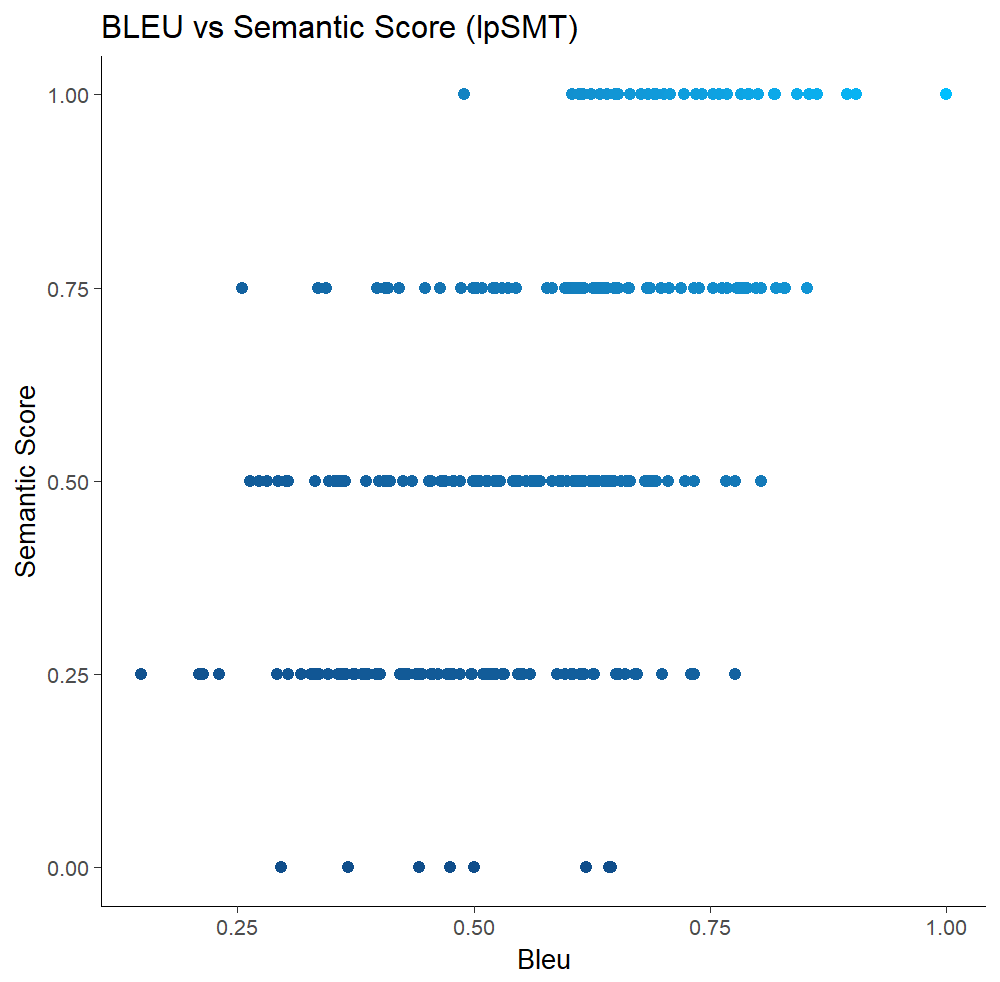
\includegraphics{img/bleuvssemantic_lpSMT.png}
\label{fig:BleuSemlpSMT}
\end{figure}

\begin{figure}
\caption{BLEU vs Semantic (mppSMT)}
\centering
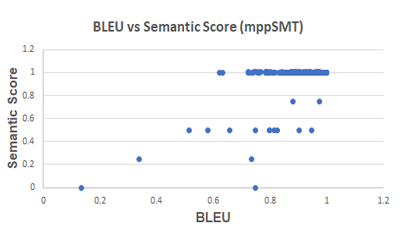
\includegraphics{img/bleuvssemantic_mppSMT.png}
\label{fig:BleuSemMppSMT}
\end{figure}

\subsection{RQ2: SED vs Semantic}
Figures \ref{fig:SedSemlpSMT}, \ref{fig:SedSemMppSMT}  show the scatter plots between 2 metrics: SED and Semantic. Each point represents scores of a pair of methods where its x-axis value is SED score and y-axis value is Semantic score.
The correlation coefficient between SED and Semantic score for the model mppSMT is 0.549 and for the model lpSMT is 0.675. That meant there is a positive relationship between the 2 metrics, but it is not strong since the correlation is closer to 0.5 than to 1.0.

Comparing to BLEU, SED has higher correlation with Semantic Score. The correlation coefficient increases from 0.524 to 0.549 (mppSMT), and 0.67 to 0.675. Nevertheless, the improvements are insignificant that can be ignored. SED suffers the same drawback as BLEU: it does not take into consideration the structures of source code. The reason SED has higher correlation can be explained by the fact that SED would deduce more heavily if the translated method has incorrect order of lexeme tokens. In a word, it is not worth to use SED instead of BLEU since it still has the same problems as BLEU. 

\begin{figure}
\caption{SED vs Semantic (lpSMT)}
\centering
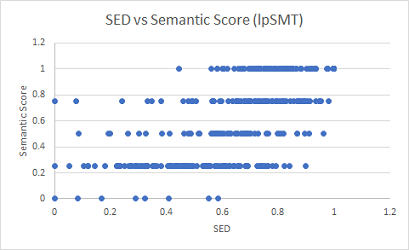
\includegraphics{img/sedvssem_lpSMT.png}
\label{fig:SedSemlpSMT}
\end{figure}

\begin{figure}
\caption{SED vs Semantic (mppSMT)}
\centering
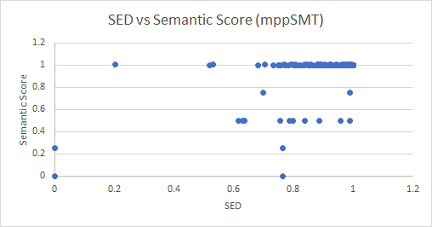
\includegraphics{img/sedvssem_mppSMT.png}
\label{fig:SedSemMppSMT}
\end{figure}

\subsection{RQ3: TREED vs Semantic}
Figures \ref{fig:TREEDlpSMT}, \ref{fig:TREEDmppSMT}  show the scatter plots between 2 metrics: TREED and Semantic. Each point represents scores of a pair of methods where its x-axis value is TREED score and y-axis value is Semantic score.
The correlation coefficient between TREED and Semantic score for the model mppSMT is 0.684 and for the model lpSMT is 0.670. That meant there is a positive relationship between the 2 metrics, but it is not strong since the correlation is closer to 0.5 than to 1.0.

\emph{Observation 1:} For a fixed value of Semantic score, there can be many associated TREED values. Specifically, in the model lpSMT, with a Semantic Score of 1, the TREED scores can be varied greatly between 0-1, which was reflected on the top horizontal line of dots in figure \ref{fig:TREEDlpSMT}. Similarly, in the figure \ref{fig:TREEDmppSMT}, with a Semantic Score of 1, the TREED scores are in the range of 0.7 to 1. 

\emph{Observation 2:} For a fixed value of TREED, there can be many associated Semantic scores. For example, the figure \ref{fig:TREEDlpSMT} shows that for a high TREED score, for example 0.8, can have Semantic Score from 0.25 to 1. This can be observed by the vertical line of dots in the figure. 

\emph{Observation 3:} TREED shows some noticeable improvement on the correlation with Semantic score on mppSMT model (0.524 to 0.684). Comparing figure \ref{fig:BleuSemMppSMT} and figure \ref{fig:TREEDmppSMT}, it can be realized that on the model mppSMT, those horizontal lines of dots in figure \ref{fig:BleuSemMppSMT} became shorter in figure \ref{fig:TREEDmppSMT}. It means the variation of TREED score for certain Semantic score is lower. Data points in the figure can also be approximately fitted with a regression line even though there still are some outliers. 

%From observation 1, it can be implied that a translated method can have low TREED score, but high Semantic score. On the other hand, from observation 2, a translated method can have high TREED score, but low Semantic score. The two implications above shows that an improvement in TREED is not sufficient nor necessary to improve translation migration quality. However, from observation 3, there is hint of positive improvement that using TREED would reflect Semantic score better than BLEU. 
From observation 1 and 2, TREED still suffers the same problem with BLEU even though the reason is different for the two metrics. A translated method can be perfectly compilable, but still fails to capture same functionality as of the reference one. 

 
\begin{figure}
\caption{TREED vs Semantic (lpSMT)}
\centering
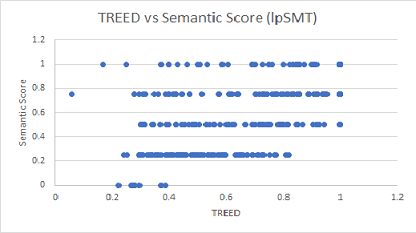
\includegraphics{img/treed_lpSMT.png}
\label{fig:TREEDlpSMT}
\end{figure}

\begin{figure}
\caption{TREED vs Semantic (mppSMT)}
\centering
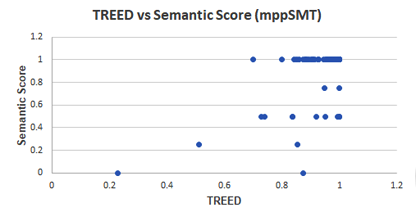
\includegraphics{img/treed_mppSMT.png}
\label{fig:TREEDmppSMT}
\end{figure}

\subsection{RQ4: GVED vs Semantic}
Figures \ref{fig:GVEDlpSMT}, \ref{fig:GVEDmppSMT}  show the scatter plots between 2 metrics: GVED and Semantic when GVED is applicable. Each point represents scores of a pair of methods where its x-axis value is GVED score and y-axis value is Semantic score. There are 240 such points for the model mppSMT, and 74 for lpSMT. 
The correlation coefficient between GVED and Semantic score for the model mppSMT is 0.893 and for the model lpSMT is 0.980. Those two correlations are very strong as they are very close to 1. A correlation coefficient of 1 means that for every positive increase of 1 in GVED, there is a positive increase of 1 in Semantic score. 

\emph{Observation 1:} The number of data points in figure \ref{fig:GVEDlpSMT} is small to draw conclusion about the correlation between GVED and Semantic score on this model (lpSMT) with high confidence. 

\emph{Observation 2:} GVED shows some significant improvement on the correlation with Semantic score on both models comparing to any of the other 3 metrics. All other 3 metrics have correlation coefficients with Semantic Score less than 0.7 while GVED achieves remarkable correlation coefficients of 0.893 and 0.980. 

From the observation 2, it can be seen that GVED is an obvious choice to evaluate SMT-based Code Migration systems since it reflects well the semantic accuracy of translated source code.  However, such systems always have the problem that the translated methods have too many errors that cannot be built into PDG, or even be compiled. That is why there are small number of data points in Figure \ref{fig:GVEDlpSMT}. Therefore, even though GVED is a reliable metrics, it is not always applicable.  

\begin{figure}
\caption{GVED vs Semantic (lpSMT)}
\centering
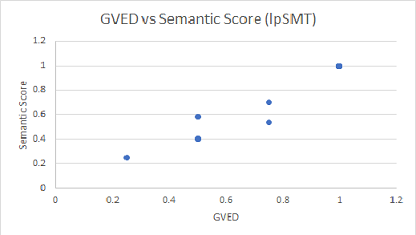
\includegraphics{img/gved_lpSMT.png}
\label{fig:GVEDlpSMT}
\end{figure}

\begin{figure}
\caption{GVED vs Semantic (mppSMT)}
\centering
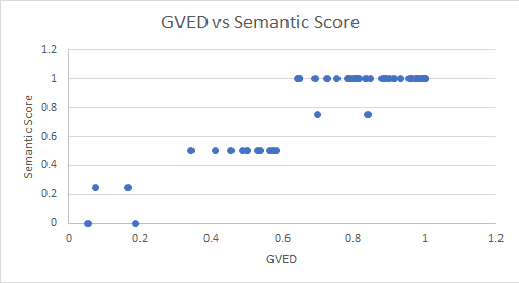
\includegraphics{img/gved_mppSMT.png}
\label{fig:GVEDmppSMT}
\end{figure}